% Standalone pipeline figure for the paper.
% Compile with: tectonic docs/figs/pipeline.tex
% Produces a tightly-cropped PDF; convert to SVG with `pdftocairo -svg`.
\documentclass[tikz,border=4pt]{standalone}
\usepackage{tikz}
\usepackage{amsmath}
\usepackage{amssymb}
\usepackage{xcolor}
\usetikzlibrary{positioning,arrows.meta,fit,backgrounds,calc}

\begin{document}
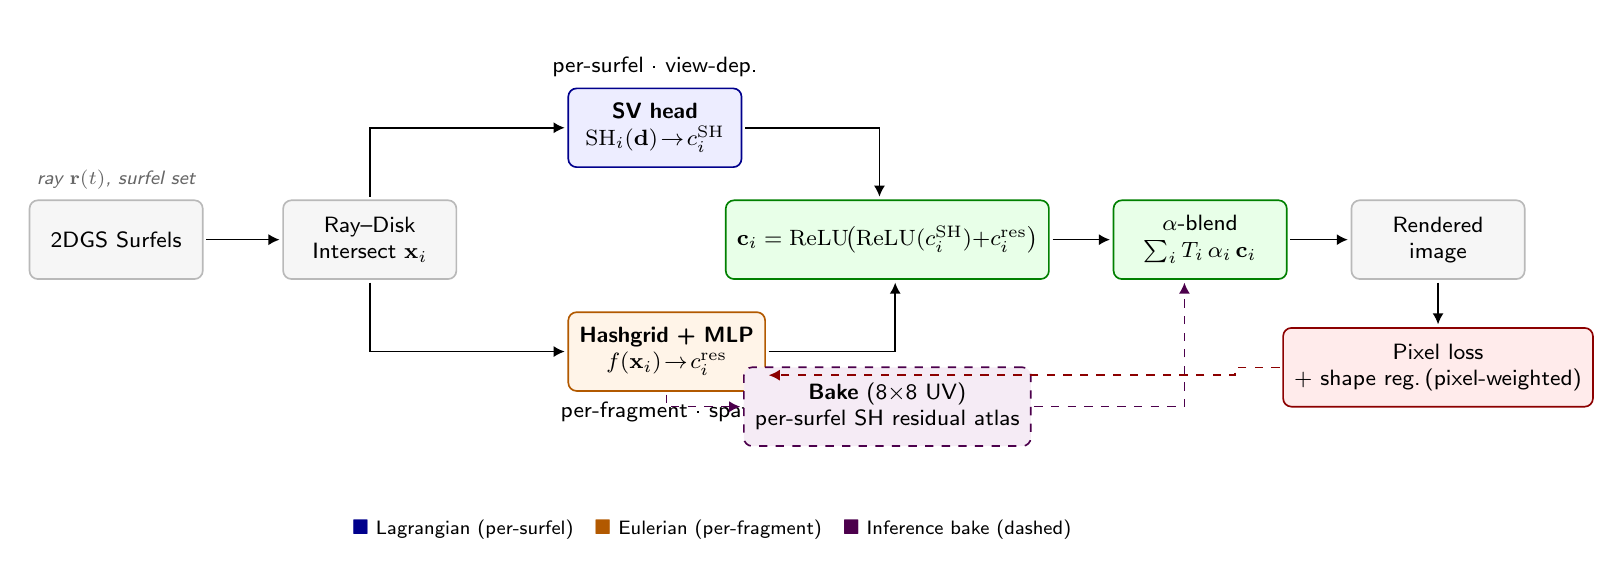
\begin{tikzpicture}[
  font=\sffamily\footnotesize,
  >={Latex[length=4pt,width=4pt]},
  thick,
  box/.style={draw, rounded corners=3pt, align=center,
              minimum height=10mm, minimum width=22mm,
              inner sep=4pt, line width=0.6pt},
  shbox/.style ={box, fill=blue!7,   draw=blue!55!black},
  mlpbox/.style={box, fill=orange!9, draw=orange!70!black},
  geo/.style   ={box, fill=gray!7,   draw=gray!55},
  blend/.style ={box, fill=green!9,  draw=green!50!black},
  loss/.style  ={box, fill=red!8,    draw=red!55!black},
  bake/.style  ={box, fill=violet!8, draw=violet!60!black, dashed},
  flow/.style  ={->, line width=0.55pt, shorten >=1pt, shorten <=1pt},
  every label/.style={font=\sffamily\scriptsize\itshape, text=black!60},
]

% inputs
\node[geo, label=above:{\scriptsize ray $\mathbf{r}(t)$, surfel set}]
  (scene) {2DGS Surfels};
\node[geo, right=10mm of scene]
  (xint)  {Ray–Disk\\Intersect $\mathbf{x}_i$};

% color paths
\node[shbox, above right=4mm and 14mm of xint]
  (sh) {\textbf{SV head}\\$\mathrm{SH}_i(\mathbf{d})\!\to\! c^{\mathrm{SH}}_i$};
\node[mlpbox, below right=4mm and 14mm of xint]
  (mlp){\textbf{Hashgrid + MLP}\\$f(\mathbf{x}_i)\!\to\! c^{\mathrm{res}}_i$};

\node[label, above=0pt of sh.north]  {per-surfel · view-dep.};
\node[label, below=0pt of mlp.south] {per-fragment · spatial};

% combine
\node[blend, right=24mm of xint.east, xshift=10mm]
  (mix) {$\mathbf{c}_i \;{=}\; \mathrm{ReLU}\!\bigl(\mathrm{ReLU}(c^{\mathrm{SH}}_i){+}c^{\mathrm{res}}_i\bigr)$};

\node[blend, right=8mm of mix]
  (alpha){$\alpha$-blend\\$\sum_i T_i\,\alpha_i\,\mathbf{c}_i$};

\node[geo, right=8mm of alpha] (img) {Rendered\\image};

% loss & reg
\node[loss, below=6mm of img]
  (loss) {Pixel loss\\$+$ shape reg.\,(pixel-weighted)};

% bake (inference)
\node[bake, below=11mm of mix]
  (bake){\textbf{Bake} (8$\times$8 UV)\\per-surfel SH residual atlas};

\draw[flow, dashed, draw=violet!60!black]
  (mlp.south) |- (bake.west);
\draw[flow, dashed, draw=violet!60!black]
  (bake.east) -| ([xshift=-2mm]alpha.south);

% training-path arrows
\draw[flow] (scene) -- (xint);
\draw[flow] (xint)  |- (sh);
\draw[flow] (xint)  |- (mlp);
\draw[flow] (sh.east)  -| ([xshift=-1mm]mix.north);
\draw[flow] (mlp.east) -| ([xshift=1mm]mix.south);
\draw[flow] (mix)   -- (alpha);
\draw[flow] (alpha) -- (img);
\draw[flow] (img)   -- (loss);

% reg backedge to shape
\draw[flow, draw=red!55!black, dashed]
  (loss.west) -- ++(-6mm,0) |- ([yshift=-3mm]mlp.east);

% legend
\node[anchor=west, font=\sffamily\scriptsize, below=8mm of bake.south west, xshift=-4mm]
{\textcolor{blue!55!black}{$\blacksquare$}~Lagrangian (per-surfel)\quad
 \textcolor{orange!70!black}{$\blacksquare$}~Eulerian (per-fragment)\quad
 \textcolor{violet!60!black}{$\blacksquare$}~Inference bake (dashed)};

\end{tikzpicture}
\end{document}
